% -*- latex -*-
%%%%%%%%%%%%%%%%%%%%%%%%%%%%%%%%%%%%%%%%%%%%%%%%%%%%%%%%%%%%%%%%
%%%%%%%%%%%%%%%%%%%%%%%%%%%%%%%%%%%%%%%%%%%%%%%%%%%%%%%%%%%%%%%%
%%%%
%%%% This text file is part of the source of 
%%%% 'Parallel techniques'
%%%% by Ángel de Vicente, copyright 2019
%%%%
%%%% TO DO:
%%%%
%%%% barnes-hut-code.tex : implementation of the Barnes-Hut algorithm
%%%%
%%%%%%%%%%%%%%%%%%%%%%%%%%%%%%%%%%%%%%%%%%%%%%%%%%%%%%%%%%%%%%%%
%%%%%%%%%%%%%%%%%%%%%%%%%%%%%%%%%%%%%%%%%%%%%%%%%%%%%%%%%%%%%%%%

\listing{barnes-hut\_serial.f90}{chapters/code/barnes-hut_serial.f90}


\begin{figure}[!htbp]
  \centering
  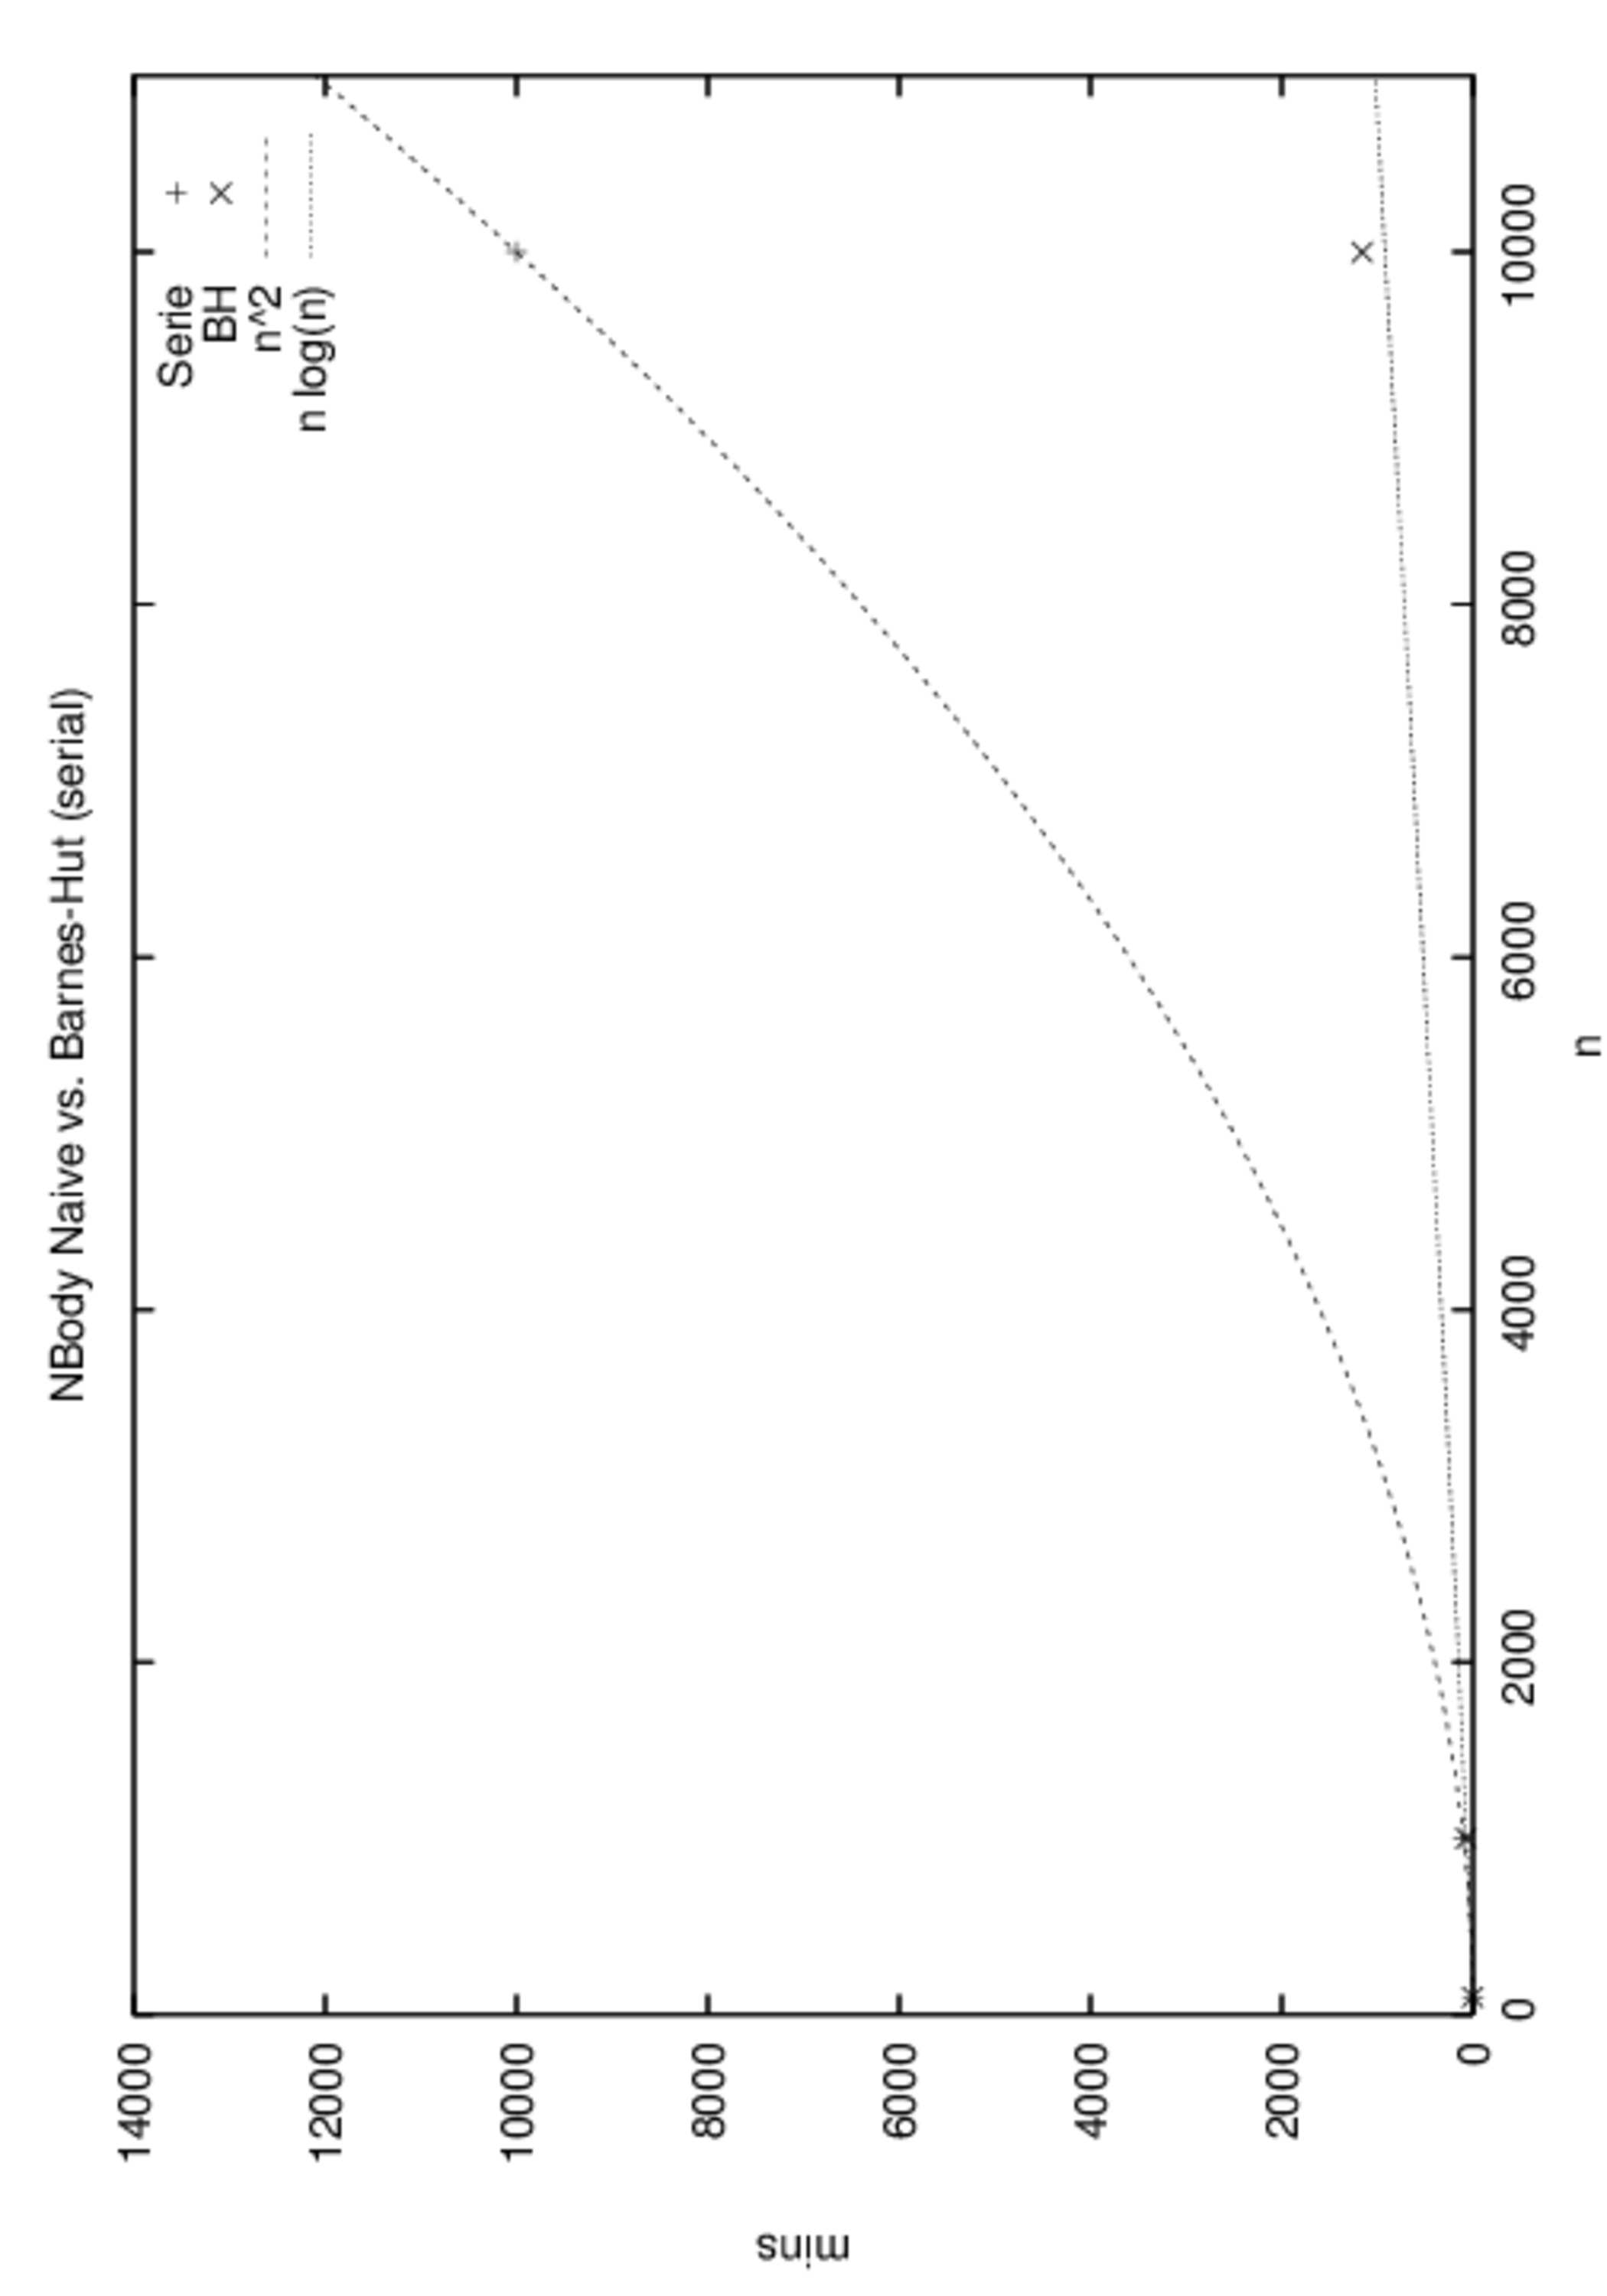
\includegraphics[angle=270,origin=c,width=0.7\textwidth]{graphics/rendimiento1.png}
  \label{fig:perf-bh-1}
  \caption{Performance Barnes Hut (1)}
\end{figure}


\begin{figure}[!htbp]
  \centering
  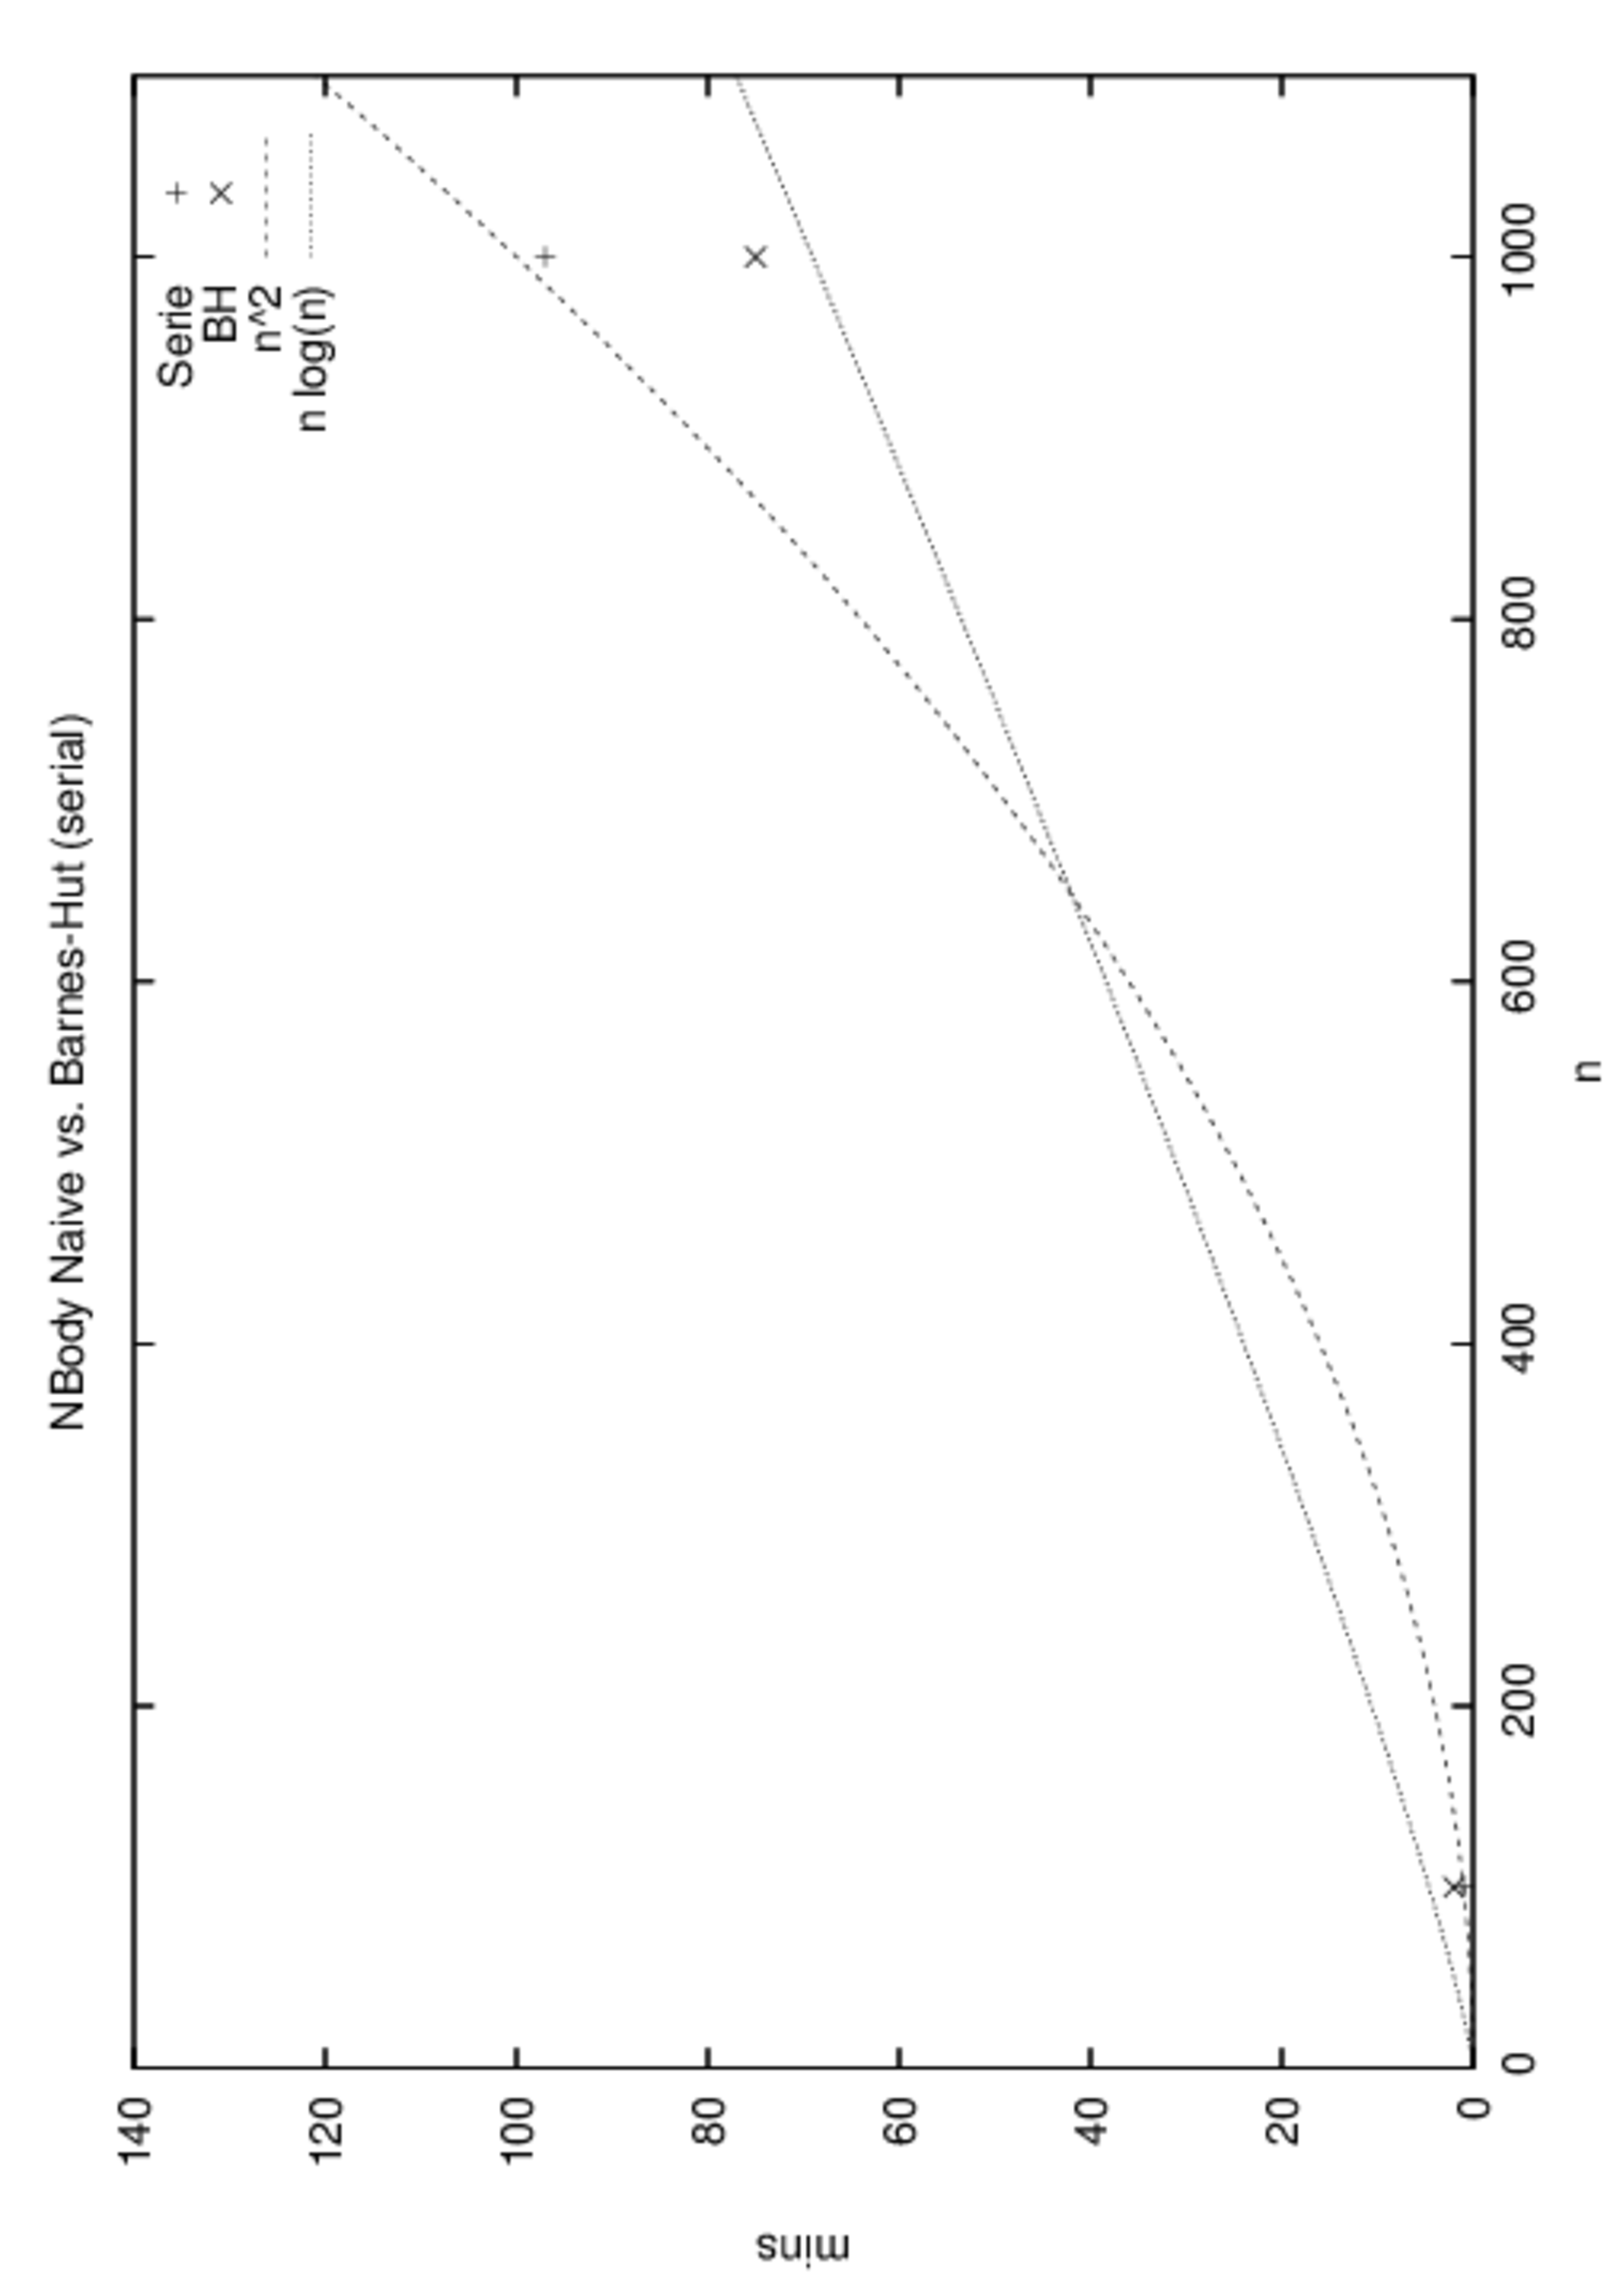
\includegraphics[angle=270,origin=c,width=0.7\textwidth]{graphics/rendimiento2.png}
  \label{fig:perf-bh-2}
  \caption{Performance Barnes Hut (2)}
\end{figure}

\begin{figure}[!htbp]
  \centering
  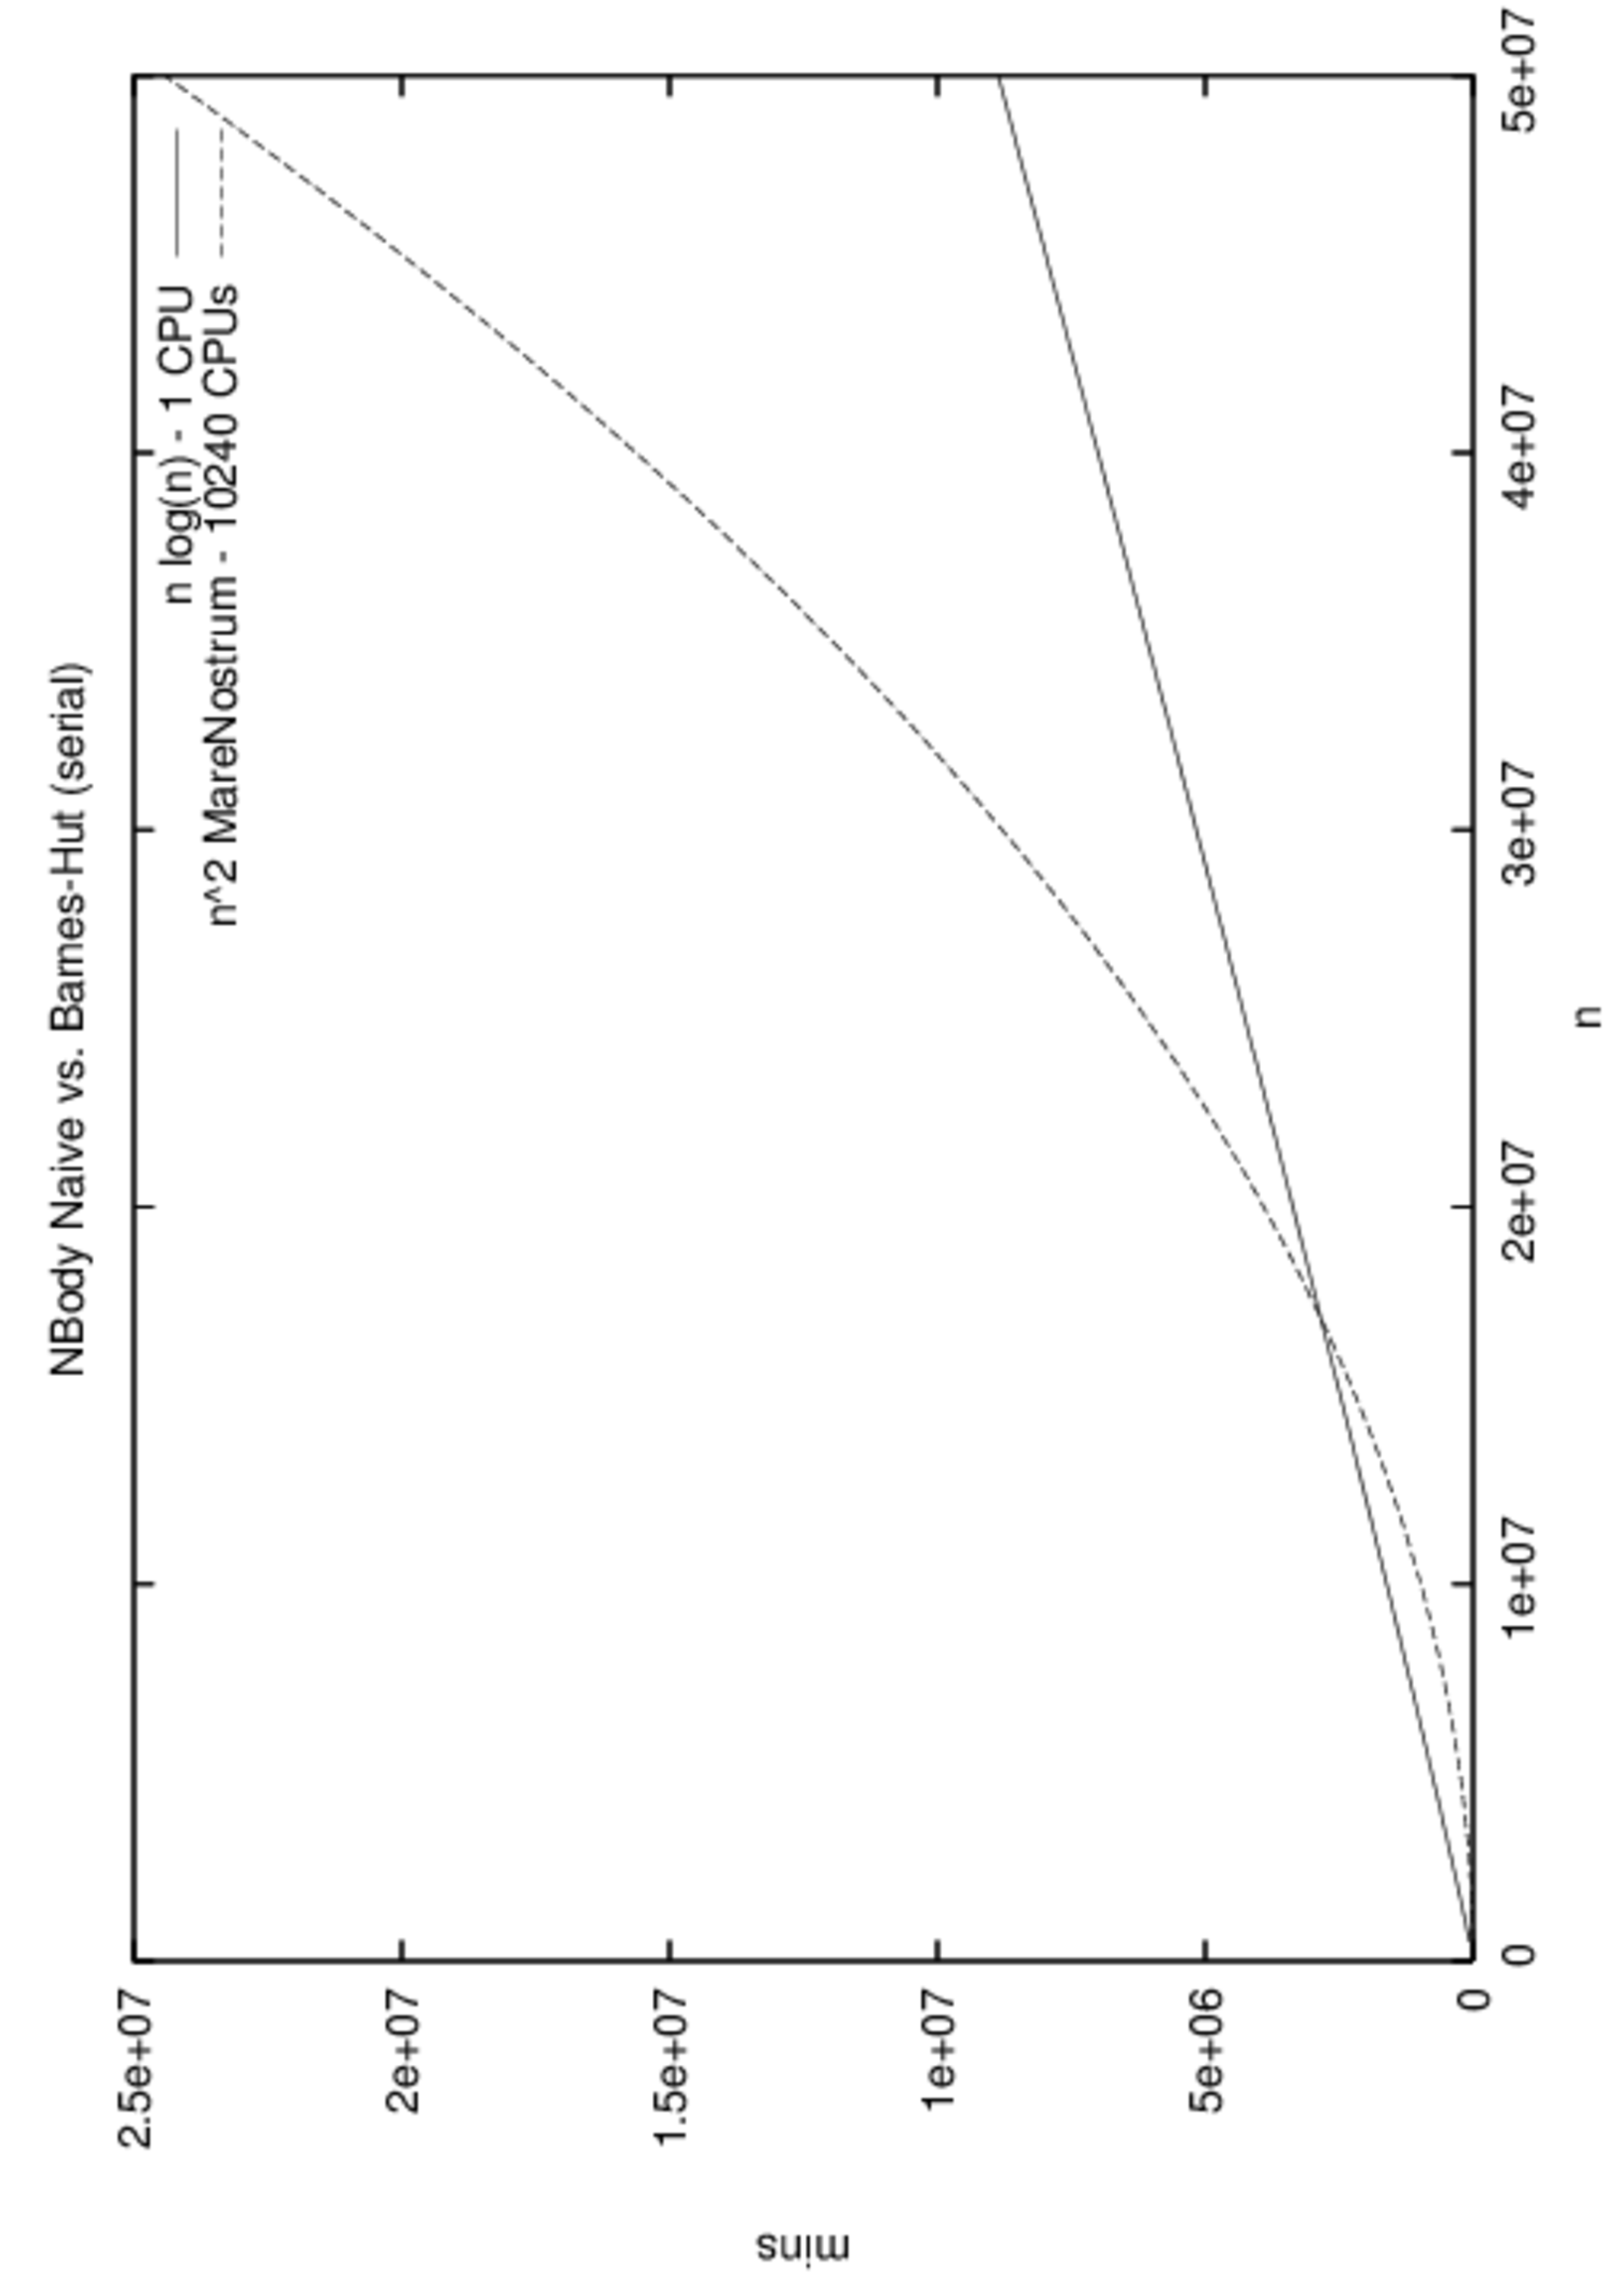
\includegraphics[angle=270,origin=c,width=0.7\textwidth]{graphics/rendimiento3.png}
  \label{fig:perf-bh-3}
  \caption{Performance Barnes Hut (3)}
\end{figure}


